\chapter{Instanciación del framework: Caso de uso}

En esta sección se presenta un caso de uso del framework Samplers tomando como ejemplo una app de ciencia ciudadana que ya se encuentra en funcionamiento, que es AppEAR, y se generará una versión usando Samplers, haciendo una breve comparación entre ambas.

\section{AppEAR}
AppEAR un sistema de ciencia ciudadana para cuidar y aprender de los ambientes acuáticos en Argentina, realizado por Joaquín Cochero, investigador del CONICET en el Instituto Platense de Limnología. Los científicos ciudadanos interactúan y colaboran en el proyecto de varias maneras, mientras que aprenden sobre los ambientes y responden a objetivos científicos. El objetivo final de AppEAR es tener un relevamiento completo y detallado de las aguas continentales de todo el territorio nacional para conocer los lugares en riesgo en los que urge trabajar. 

Los voluntarios de este proyecto descargan una aplicación para su dispositivo móvil y toman muestras para el proyecto. La aplicación guía a los usuarios a través de los pasos necesarios para tomar una muestra.\cite{appEar}

\begin{figure}[H]
  \centering
   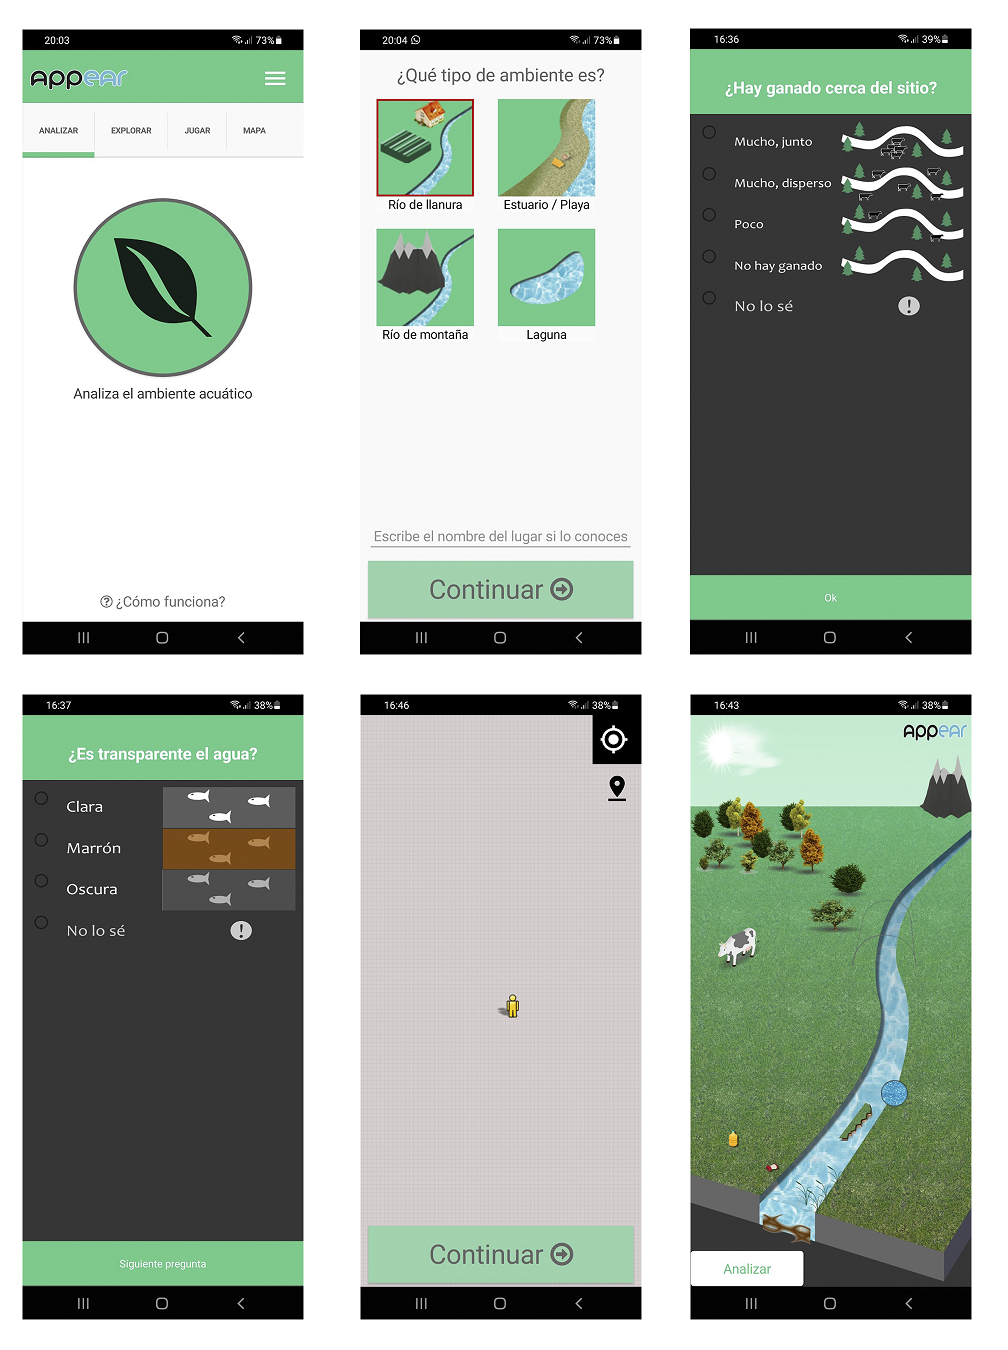
\includegraphics[scale=0.5]{06-caso_de_uso/capturas_appear.png} 
    \caption{Capturas de pantalla de la app AppEAR}
\end{figure}

Como se mencionó antes, la app va guiando a los científicos ciudadanos a través de los pasos necesarios para tomar una muestra, que son básicamente preguntas acerca del lugar que están relevando y de las cosas que ven alrededor. AppEAR diferencia 4 tipos de ambientes, que son río de llanura, río de montaña, estuario/playa y laguna, y en base a eso realiza algunas preguntas que son específicas de cada tipo y el resto preguntas comunes a los 4 tipos de ambientes. A medida que se van completando las preguntas, la app va armando una especie de dibujo del lugar con figuras que representan los elementos observados por el científico ciudadano.

Analizando todos los pasos propuestos por AppEAR se puede deducir el Workflow para tomar la muestra representado en el siguiente grafo direccional:

\begin{figure}[H] \label{img_grafo_appear}
  \centering
   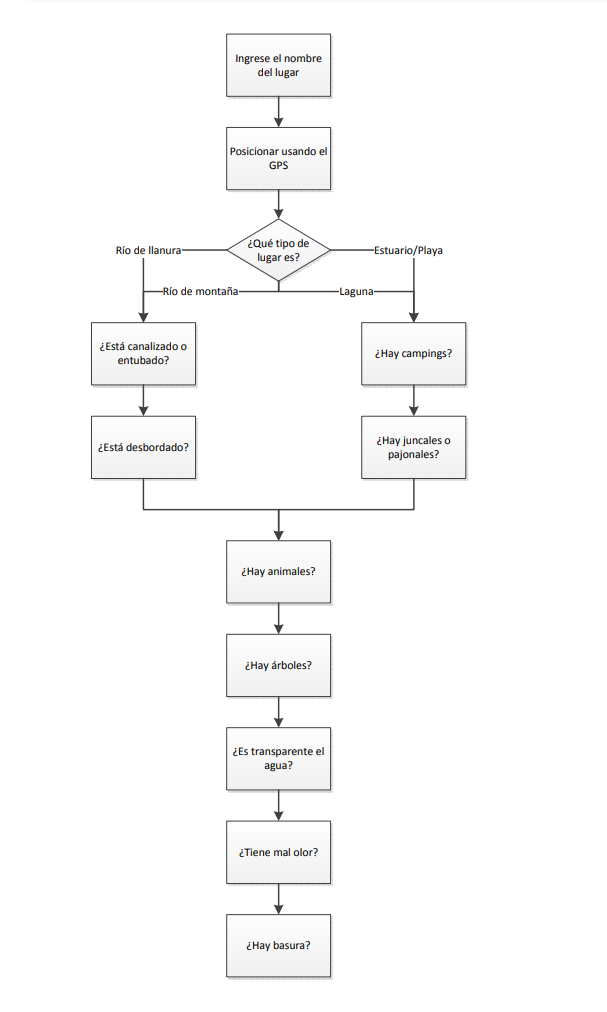
\includegraphics[scale=0.65]{06-caso_de_uso/flujo_appear.png} 
    \caption{Grafo direccional que representa el Workflow de AppEAR}
\end{figure}

\section{AppEar usando Samplers}
A continuación se muestra como sería AppEAR usando Samplers.

Observando el Workflow planteado en la figura \ref{img_grafo_appear}, se genera el archivo de configuración para Samplers de la siguiente manera:

\begin{figure}[H]
  \centering
   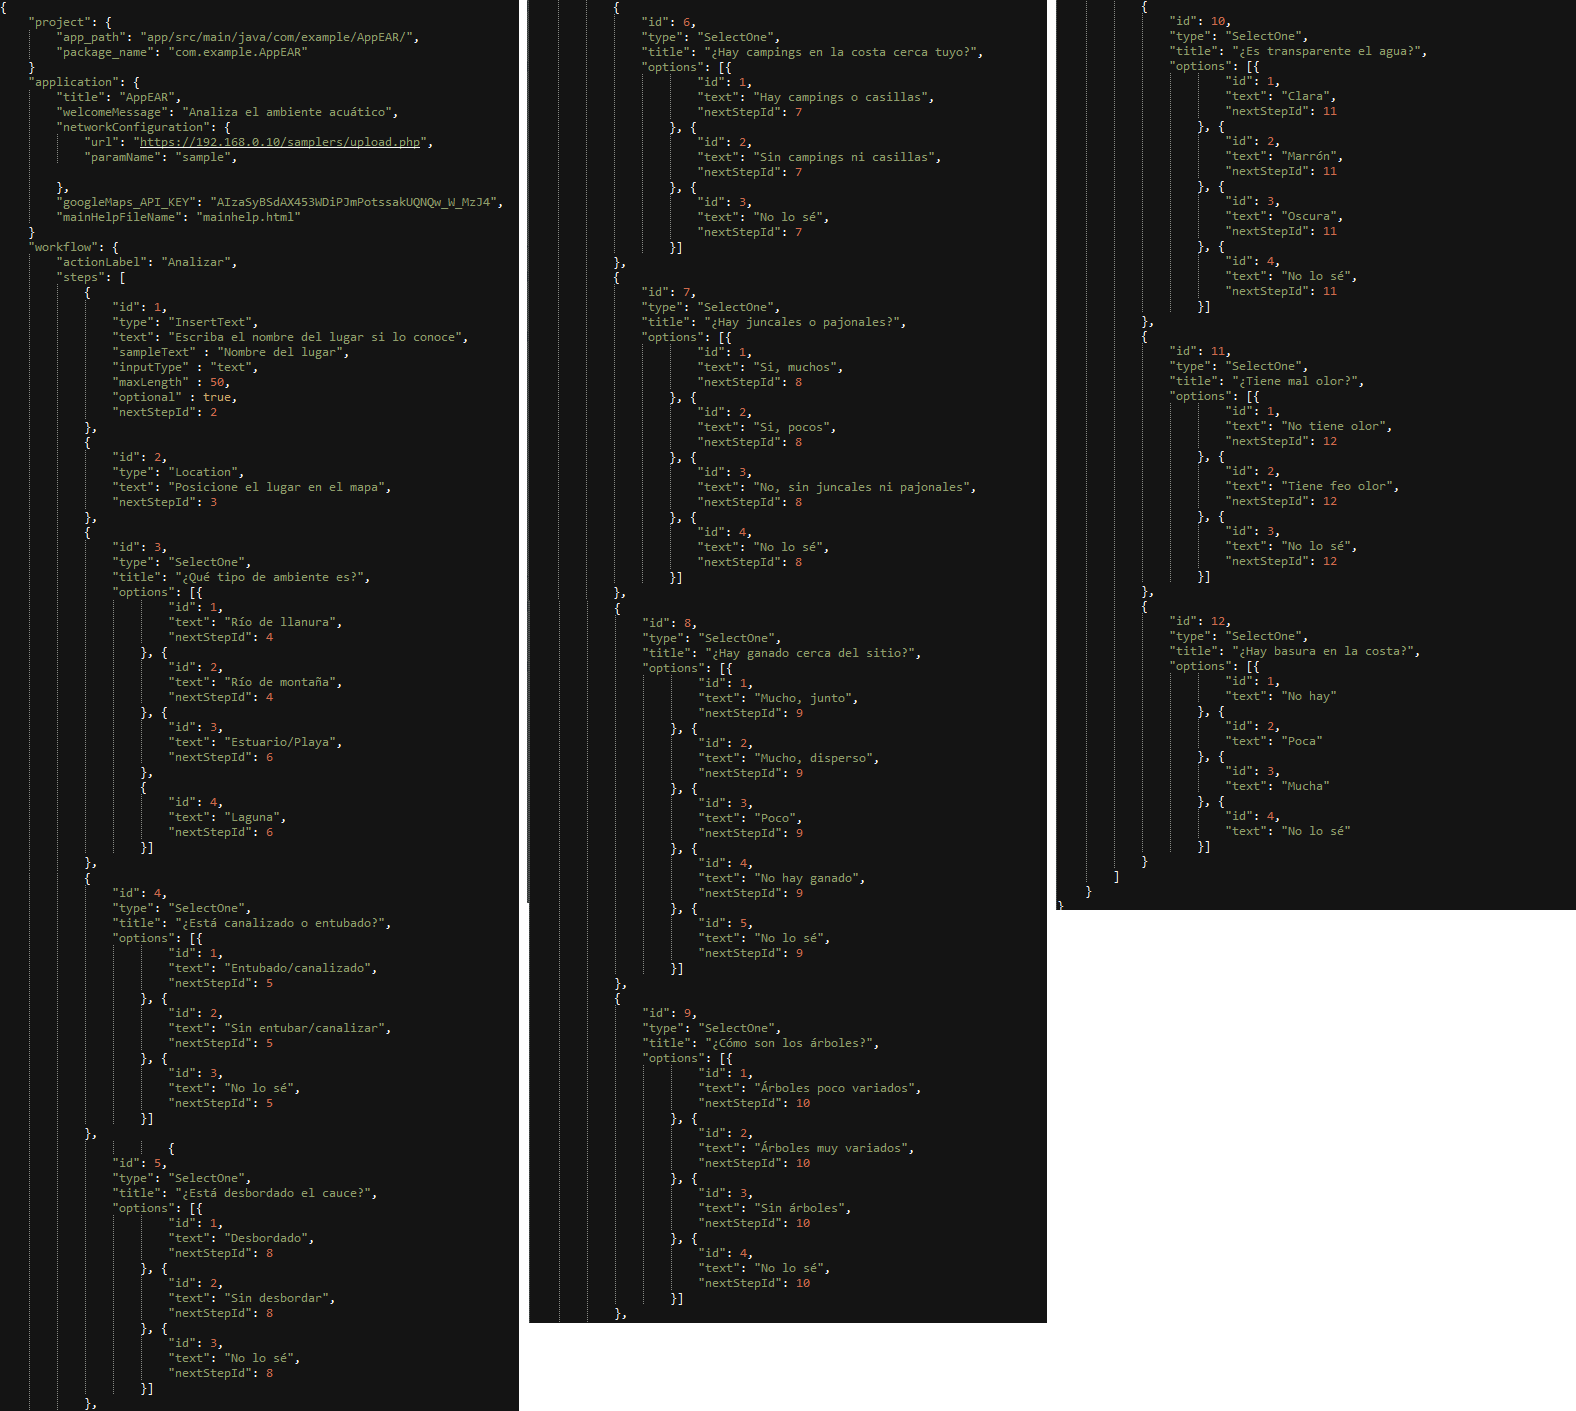
\includegraphics[scale=0.3]{06-caso_de_uso/archivo_configuracion.png} 
    \caption{Archivo de configuración para Samplers para generar una app equivalente a AppEAR}
\end{figure}

Una vez completado el archivo de configuración, se ejecuta Samplers y se genera la app.

\begin{figure}[H]
  \centering
   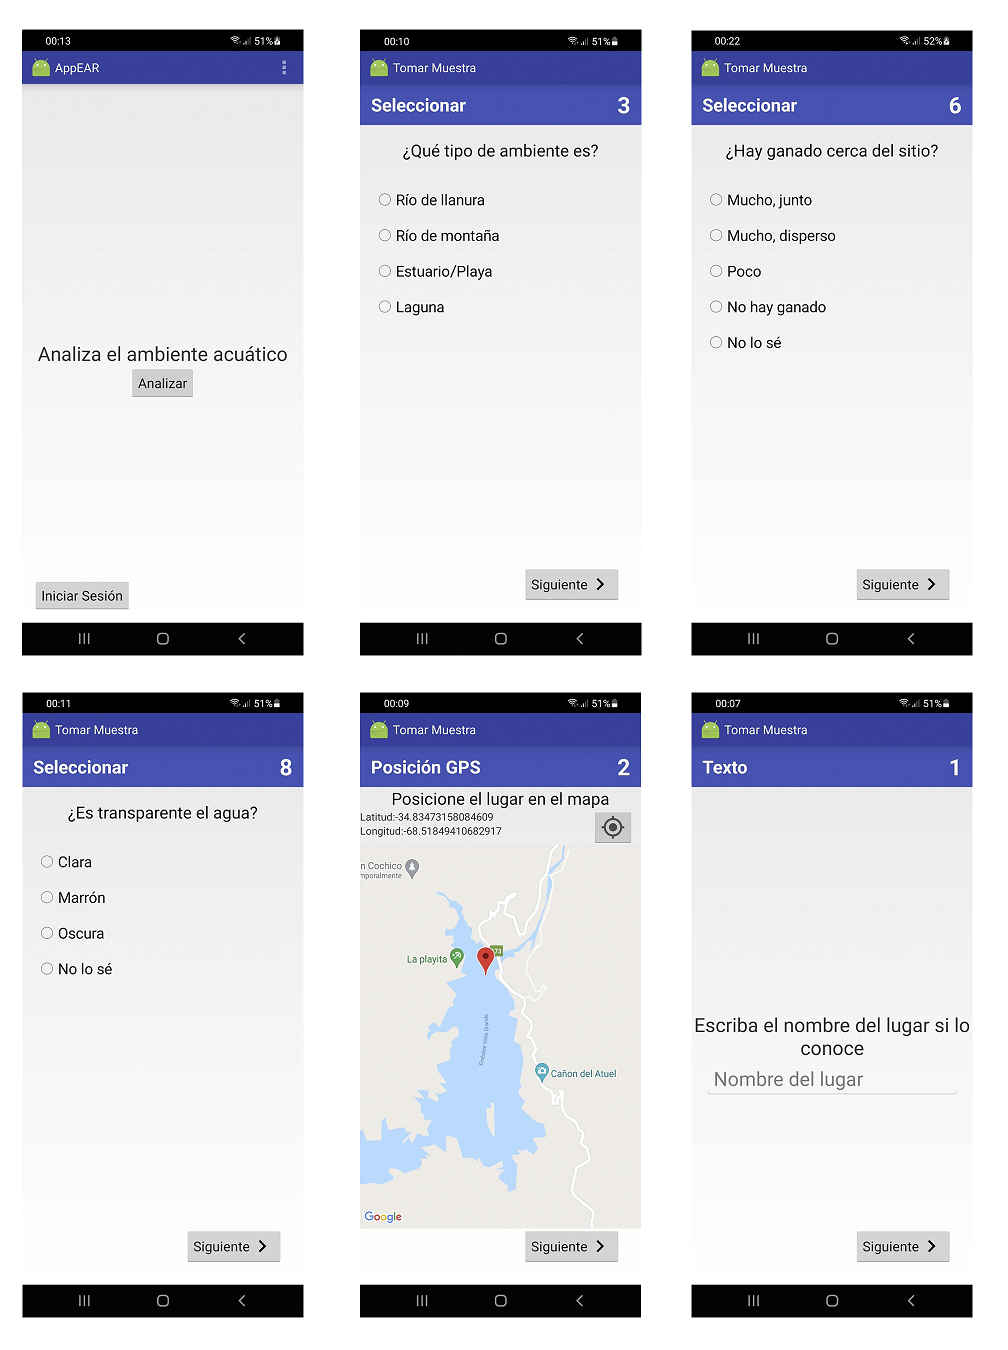
\includegraphics[scale=0.5]{06-caso_de_uso/capturas_appear_samplers.png} 
    \caption{Capturas de pantalla de la app AppEAR generada por Samplers}
\end{figure}

\section{Comparación y conclusión}
[breve comparacion y conclusion]